\chapter{Introduction}
\markboth{Introduction}{}% To set left/right header
% \localtableofcontents

\section{Robust Control-Aware Motion Planning}

\section{Context and Objectives}

\begin{figure} [t]
    \centering
    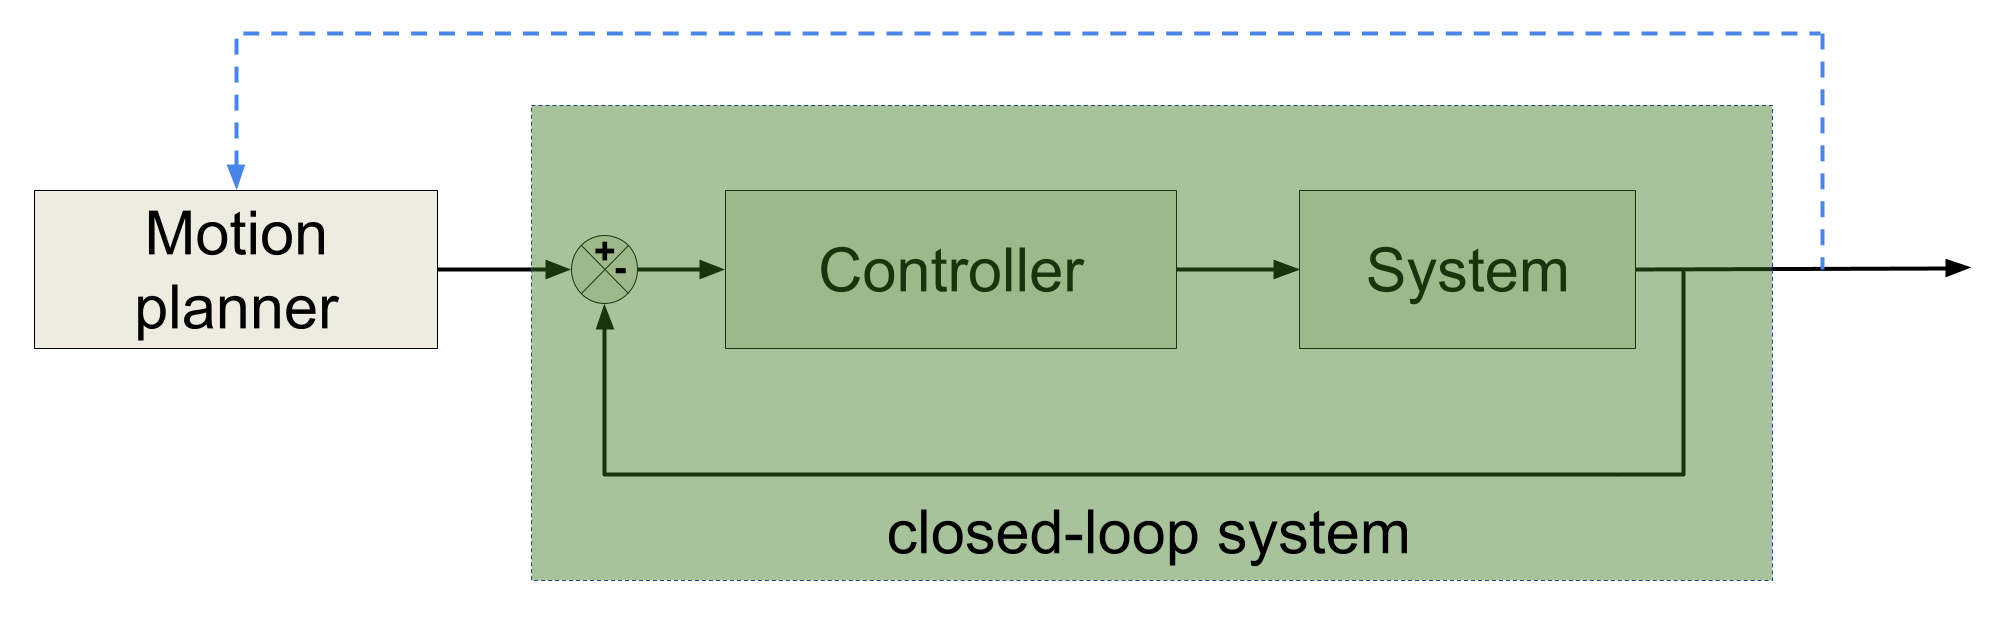
\includegraphics[width=0.9\linewidth]{figures/intro/control-aware.png} 
    \caption{Illustration of the control-aware motion planning strategy.
    It relies on the closed-loop system simulation (green) at the offline motion planning level (gray).}%
    \label{fig:ca_strat}%
  \end{figure}

\section{Thesis Outline}

This manuscript begins with a literature review in Chapter~\ref{chap:related_work}, providing an overview of the current state of the art. 
It initially focuses on decoupled approaches to robust motion planning, starting with path finding methods and progressing to kinodynamic planning paired with robust control strategies.
The review then continues to unified approaches, presenting robust motion planning methods that address uncertainty, as well as control-aware planning techniques. 
The chapter concludes with a focus on unified robust control-aware motion planning approaches, which form the main topic of interest.

Chapter~\ref{chap:models} introduces the \emph{closed-loop sensitivity} concept and present how this concept can be leveraged to derive the so-called uncertainty tubes.
These uncertainty tubes are later employed in this thesis to impose robust constraints on systems while accounting for parametric uncertainties.
Then, this chapter presents the quadrotor and differential drive robot models considered in this thesis, along with their respective controllers and local planning techniques used for generating reference trajectories.

The first contribution of this thesis is then introduced in Chapter~\ref{chap:samp}.
It presents the general method for integrating sensitivity-based uncertainty tubes into sampling-based planners to create various sensitivity-aware motion planner variants.
Furthermore, this chapter emphasizing the generation of sensitivity-optimal trajectories in global context.
Initial simulation results, using the models introduced in Chapter~\ref{chap:models}, highlight that computing uncertainty tubes become a bottleneck for sampling-based methods.
To address this, a more efficient variant is proposed, leveraging a lazy collision-checking approach to reduce the frequency of uncertainty tube computations.

Chapter~\ref{chap:NN} introduces the second major contribution of this thesis, which leverages the structural similarities between ordinary differential equations and recurrent neural network cells to accelerate the computation of sensitivity-based uncertainty tubes. 
A dataset generation method, based on sampling-based principle, is proposed and applied to the models discussed in Chapter~\ref{chap:models}. 
The method achieves an optimal balance between inference time and accuracy, making it highly effective for motion planning and showcasing the efficiency of the approach.

Chapter~\ref{chap:sampNN} aims to integrate the sensitivity-aware motion planning variants introduced in Chapter~\ref{chap:samp} with the deep learning approach detailed in Chapter~\ref{chap:NN}, resulting in a more efficient version of the sensitivity-aware motion planner variants.
Furthermore, while the previous chapters solely focus on generating robust and sensitivity-optimized trajectories, this chapter emphasizes the generation of task-specific accurate trajectories.
The effectiveness of this contribution is finally demonstrated through experimental validation on two challenging scenarios.

\section{Thesis Contributions}

The work conducted throughout this thesis led to the following publications in international peer-reviewed conferences and letters. 

~\cite{cSAMP} Wasiela, S., Giordano, P. R., Cortés, J., and Simeon, T. (2023, May). "A sensitivity-aware motion planner (samp) to generate intrinsically-robust trajectories." In IEEE International Conference on Robotics and Automation (ICRA) (pp. 12707-12713).

~\cite{cECAI}: Wasiela, S., Bouhsain, S. A., Cognetti, M., Cortés, J., and Simeon, T. (2024, October). "Learned Uncertainty Tubes via Recurrent Neural Networks for Planning Robust Robot Motions." In 27th European Conference on Artificial Intelligence (ECAI) (pp. 4385-4392).

~\cite{cRAL}: Wasiela, S., Cognetti, M., Giordano, P. R., Cortés, J., and Simeon, T. (2024). "Robust Motion Planning with Accuracy Optimization based on Learned Sensitivity Metrics." In IEEE Robotics and Automation Letters (RA-L).

Furthermore, all implementations presented and used in this thesis are available at: \href{https://gitlab.laas.fr/CAMP}{https://gitlab.laas.fr/CAMP}.